\documentclass[conference,nofonttune]{IEEEtran}
\usepackage{graphicx}
\usepackage{mathtools}
\usepackage{lmodern}
\usepackage{amsmath}
\usepackage{float}

%\usepackage{mathptmx} % times font
%\usepackage{helvet} % helvetica font
%\usepackage{courier} % courier font

%\usepackage{amsmath}
%\interdisplaylinepenalty=2500
%\usepackage{array}
%\usepackage{bm}
%\usepackage{latexsym}
%\usepackage{amsmath}
%\usepackage{amsfonts}
%\usepackage{amssymb}

\begin{document}
%
% paper title
% Titles are generally capitalized except for words such as a, an, and, as,
% at, but, by, for, in, nor, of, on, or, the, to and up, which are usually
% not capitalized unless they are the first or last word of the title.
% Linebreaks \\ can be used within to get better formatting as desired.
% Do not put math or special symbols in the title.
\title{Point cloud-based camera calibration for AR}


% author names and affiliations
% use a multiple column layout for up to three different
% affiliations
\author{\IEEEauthorblockN{Stefan Eichenberger}
\IEEEauthorblockA{Bern University of Applied Sciences\\ BFH-TI, CH2502-Biel, Switzerland.\\
Email: stefan.eichenberger@students.bfh.ch}}

% conference papers do not typically use \thanks and this command
% is locked out in conference mode. If really needed, such as for
% the acknowledgment of grants, issue a \IEEEoverridecommandlockouts
% after \documentclass

% for over three affiliations, or if they all won't fit within the width
% of the page, use this alternative format:
%
%\author{\IEEEauthorblockN{Michael Shell\IEEEauthorrefmark{1},
%Homer Simpson\IEEEauthorrefmark{2},
%James Kirk\IEEEauthorrefmark{3},
%Montgomery Scott\IEEEauthorrefmark{3} and
%Eldon Tyrell\IEEEauthorrefmark{4}}
%\IEEEauthorblockA{\IEEEauthorrefmark{1}School of Electrical and Computer Engineering\\
%Georgia Institute of Technology,
%Atlanta, Georgia 30332--0250\\ Email: see http://www.michaelshell.org/contact.html}
%\IEEEauthorblockA{\IEEEauthorrefmark{2}Twentieth Century Fox, Springfield, USA\\
%Email: homer@thesimpsons.com}
%\IEEEauthorblockA{\IEEEauthorrefmark{3}Starfleet Academy, San Francisco, California 96678-2391\\
%Telephone: (800) 555--1212, Fax: (888) 555--1212}
%\IEEEauthorblockA{\IEEEauthorrefmark{4}Tyrell Inc., 123 Replicant Street, Los Angeles, California 90210--4321}}




% use for special paper notices
%\IEEEspecialpapernotice{(Invited Paper)}




% make the title area
\maketitle

% As a general rule, do not put math, special symbols or citations
% in the abstract
\begin{abstract}
  To reconstruct the pose and position of a camera the intrinsic camera model must once be calculated. We show a method on how to calibrate a camera based on a pregenerated point cloud. This method makes camera calibration more user friendly for augmented reality applications where pregenerated point clouds can be used.
\end{abstract}

% no keywords

% For peer review papers, you can put extra information on the cover
% page as needed:
% \ifCLASSOPTIONpeerreview
% \begin{center} \bfseries EDICS Category: 3-BBND \end{center}
% \fi
%
% For peerreview papers, this IEEEtran command inserts a page break and
% creates the second title. It will be ignored for other modes.
\IEEEpeerreviewmaketitle

\section{Introduction}
Augmented Reality (AR) overlays computer-generated images over the real world. It is well-known that the perceived quality of AR-applications strongly depends on reliable camera modeling and parameter calibration \cite{Zaun}. Today’s AR platforms have stored the parameters of the camera model on the filesystem. This is possible because the manufacturer knows the exact type of the camera. Here, we choose a different approach and calibrate the camera "on the fly" in a given and partially known environment. This on the fly calibration extends the classic approach of checkerboard calibration \cite{Zhang} (Figure \ref{fig:checkerboard}). It is based on the knowledge of a 3d point cloud of the environment where we want to do AR.


\section{Point cloud}
For our approach, a point cloud of a given location is needed. A point cloud is a collection of points within a 3-dimensional space. We know the position (x,y,z) of each point and its unique descriptor. The descriptor must be translation and rotation invariant. The cloud can be stored in a file for future use. We chose ORB2 monocular SLAM \cite{orbslam} for this purpose because it is open source, good documented and well established. Monocular SLAM is chosen because its handling is much simpler than with other systems (e.g. stereo camera). ORB2 Slam performs the following steps:
\begin{enumerate}
\item Search distinctive points on the image e.g. corners
\item Calculate an ORB descriptor at all distinctive points
\item Calculate the translation and rotation between two views
\item Estimate the position and rotation of the image to the first keyframe
\item Calculate the position of the points regarding the position of the first keyframe
\end{enumerate}

We store the position and the ORB descriptor of each point in a file to make the point cloud persistent.\\
In theory, our approach needs 6 points to solve equation \ref{eq:cm} with 17 unknowns. To solve equation \ref{eq:dist} another 5 unknowns are added. In theory, we would need 8 points in total. In practice, more points are required to detect outliers and to reduce the influence of noise. A minimum of 30 points is well suited for our approach.

\begin{figure}
  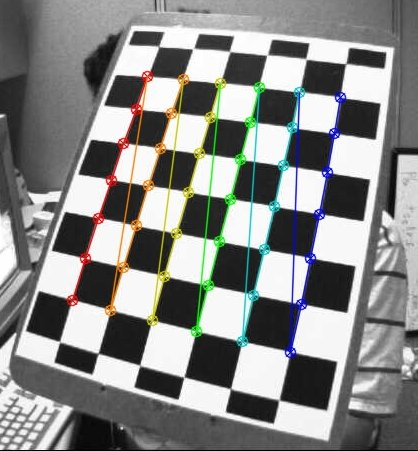
\includegraphics[width=0.5\textwidth]{img/checkerboard.jpg}
\caption{Classic calibration by checkerboard}\label{fig:checkerboard}
\end{figure}

\section{Camera Model}
For our method, we need to guess the 2d image point from the 3d world point. This can be done by the well-known camera model \cite{rac} shown in equation \ref{eq:cm}. The first matrix is called intrinsic camera matrix while the second one is called extrinsic camera matrix.
\begin{figure}
  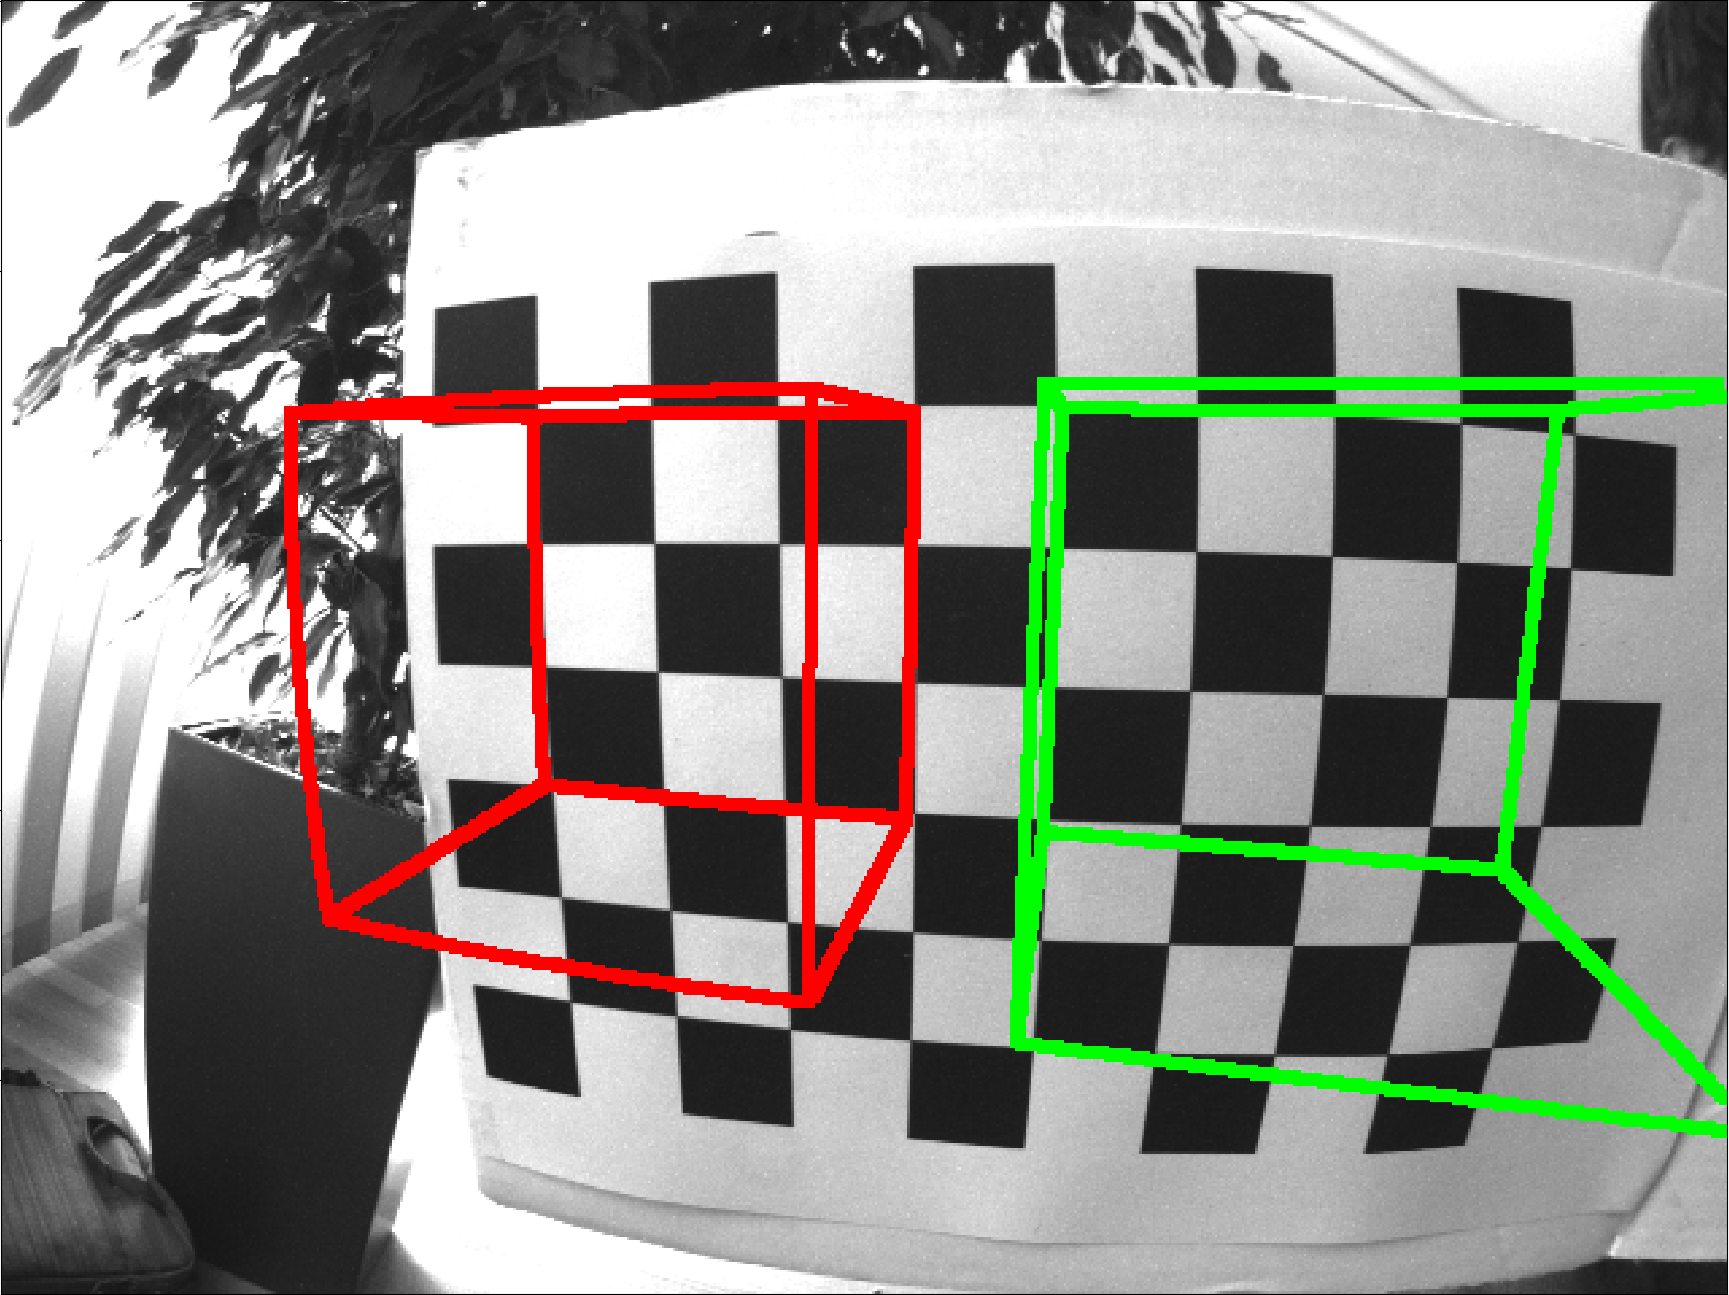
\includegraphics[width=0.5\textwidth]{img/model.png}
  \caption{Image generated from a 3d model with (right) and without (left) distortion}
  \label{fig:model}
\end{figure}
\scriptsize
\begin{equation}\label{eq:cm}
  \begin{pmatrix}fx & \gamma & cx \\
      0 & fy & cy \\
      0 & 0 & 1 \\
    \end{pmatrix}*
    \begin{pmatrix}
      r_{00} & r_{01} & r_{02} & tx \\
      r_{10} & r_{11} & r_{12} & ty \\
      r_{20} & r_{21} & r_{22} & tz \\
    \end{pmatrix}
    \begin{pmatrix}
      X \\
      Y \\
      Z \\
      1
    \end{pmatrix}=
    \begin{pmatrix}
      u \\
      v \\
      s
  \end{pmatrix}
\end{equation}
\normalsize
Where:
\begin{align*}
  X,Y,Z		&: \text{point in the 3d world}\\
  u,v	    	&: \text{point in a 2d image}\\
  s		&: \text{scaling factor (1 when normalized)}\\
  fx,fy   	&: \text{focal length of the camera}\\
  cx,cy   	&: \text{sensor displacement}\\
  tx,ty,tz	&: \text{translation with respect to the camera}\\
  r_{ij}	&: \text{part of the rotation matrix}
\end{align*}
With this equation, it is possible to generate 2d points from a 3d point cloud (Figure \ref{fig:model}).
Additional to equation \ref{eq:cm} we simulate distortion (equation \ref{eq:dist}) from the camera objective. The distortion is added to the 2d coordinates as shown in equation \ref{eq:pdist}.\\
\scriptsize
\begin{equation}\label{eq:dist}
	\begin{pmatrix}\gamma_{u} \\
	  \gamma_{v}
	\end{pmatrix}=\begin{pmatrix}
	  u(k_1r^2+k_2r^4+k_3r^6)\\
	  v(k_1r^2+k_2r^4+k_3r^6)
	\end{pmatrix}+\begin{pmatrix}
	  2p_1uv+p_2(r^2+2u^2)\\
	  p_1(r^2+2v^2)+2p_2uv
	\end{pmatrix}
\end{equation}
\begin{equation}\label{eq:pdist}
\begin{pmatrix}u'\\v'\end{pmatrix}=\begin{pmatrix}
u\\v\end{pmatrix}+\begin{pmatrix}\gamma_{u}\\\gamma_{v}\end{pmatrix}
\end{equation}
\normalsize
Where:
\begin{align*}
  k_{i}		&: \text{radial distortion}\\
  p_{i}	    	&: \text{tangential distortion}\\
  \gamma_{i}	&: \text{summed distortion}\\
  u',v'		&: \text{distorted image points}
\end{align*}


\section{Optimization}
From a given image it is possible to calculate the ORB descriptors \cite{orbslam}. These descriptors are matched against the descriptors of the point cloud. If enough matches are found it is possible to calculate the camera model parameters. This is done by minimizing the reprojection error (equation \ref{eq:reprojerr}). The reprojection error is the difference between the real 2d points and the 3d points transformed to the 2d image (equation \ref{eq:transformation}). To avoid extracting the root our mechanism uses the squared reprojection error.\\
\scriptsize
\begin{equation}\label{eq:transformation}
\begin{pmatrix}u'\\v'\end{pmatrix}=C*E*P+\gamma
\end{equation}
\begin{equation}\label{eq:reprojerr}
e=(u'-u)^2+(v'-v)^2
\end{equation}
\normalsize
Where:
\begin{align*}
  C		&: \text{intrinsic camera matrix}\\
  E	    	&: \text{extrinsic camera matrix}\\
  P		&: \text{3d point}\\
  \gamma   	&: \text{distortion}\\
  e		&: \text{reprojection error}
\end{align*}

Because the distortion is nonlinear a nonlinear solver must be used to minimize the least square problem. Zhang \cite{Zhang} has found that the Levenberg-Marquardt solver works well for this purpose. With synthetic data, the minimizer will find the original camera model. Unfortunately, the model is prone to noise as figure \ref{fig:reprojerr} shows. In reality, the distance of a point to the camera is hard to guess and the generated point cloud will therefore always be noisy.

\begin{figure}
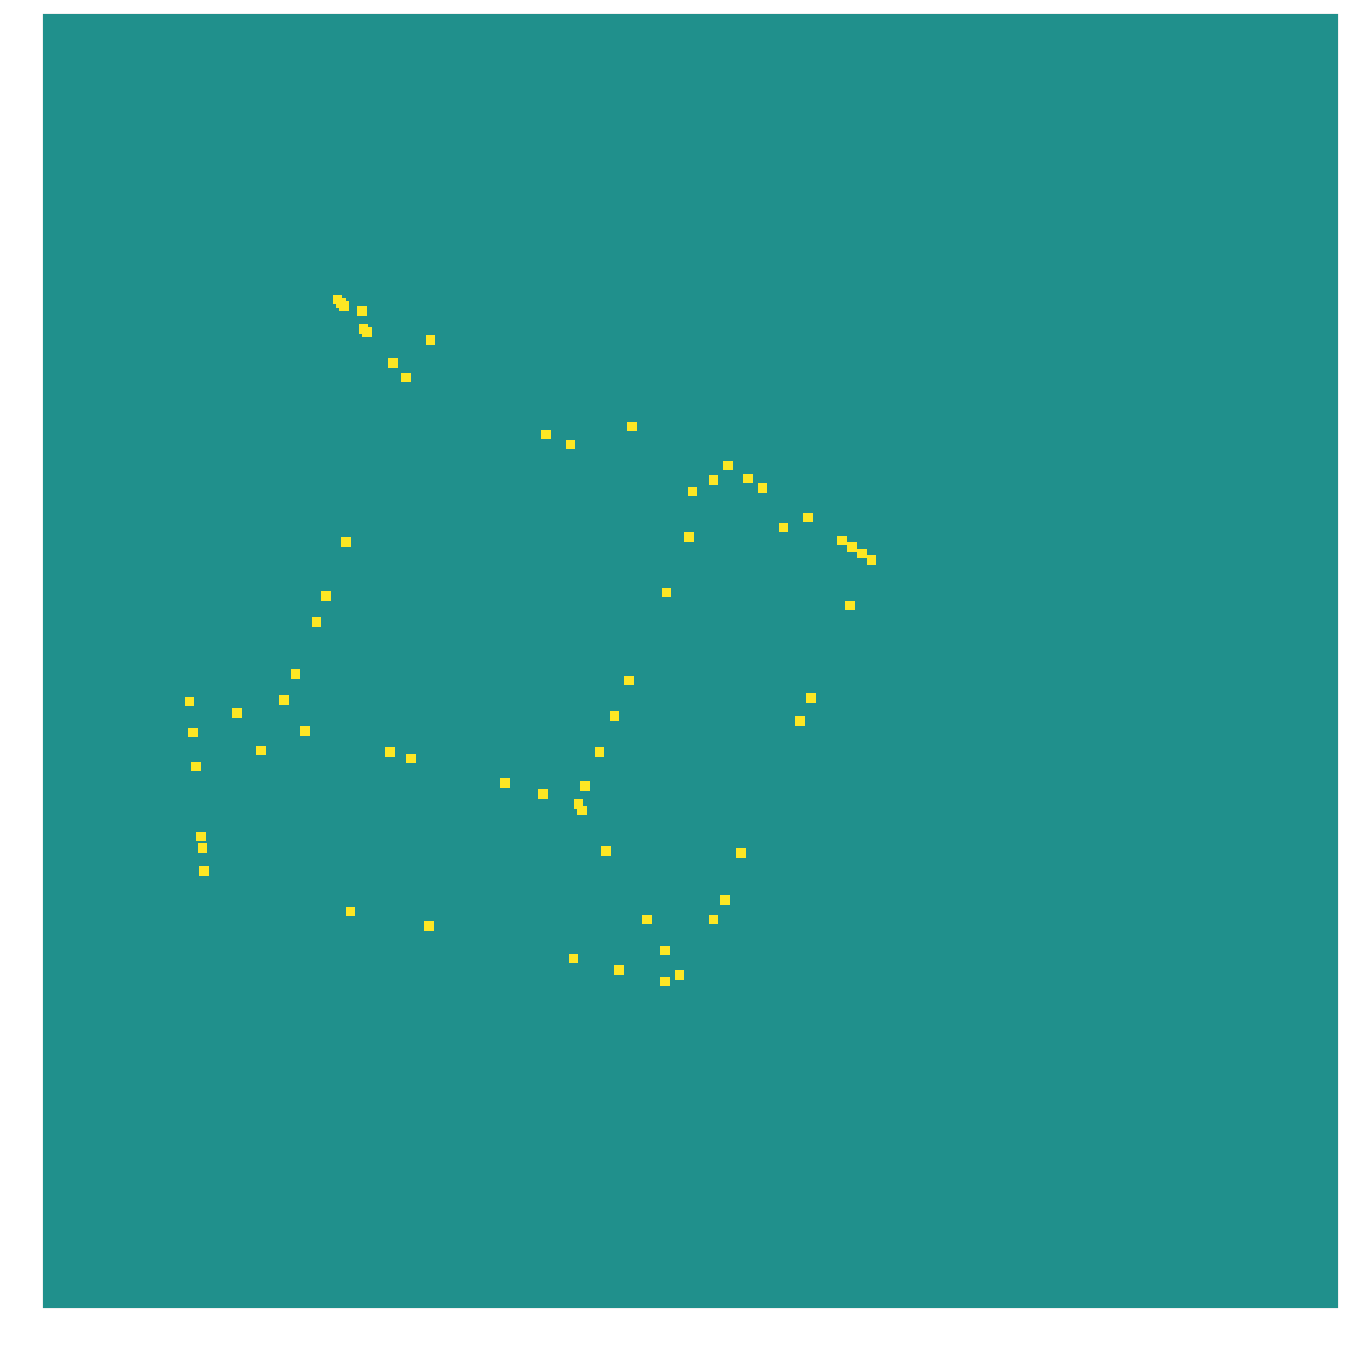
\includegraphics[width=0.5\textwidth]{img/reprojection_error.png}
\caption{Pixels that do not match after reprojection because of noise}\label{fig:reprojerr}
\end{figure}

\section{Results}
We have shown that the algorithm for point cloud-based camera calibration works in theory. Using synthetic data, we can regain the intrinsic camera matrix as well as the distortion parameters. With practical data, the main problem is to generate a precise point cloud. The algorithm is indeed sensitive to noise. Point clouds generated with a monocular SLAM system will, therefore, be hard to use for our use case.\\
To make the algorithm less prone to noise, RANSAC \cite{ransac} may be used to find outliers. The outliers can then be ignored in a second optimization step.

% can use a bibliography generated by BibTeX as a .bbl file
% BibTeX documentation can be easily obtained at:
% http://mirror.ctan.org/biblio/bibtex/contrib/doc/
% The IEEEtran BibTeX style support page is at:
% http://www.michaelshell.org/tex/ieeetran/bibtex/
%\bibliographystyle{IEEEtran}
% argument is your BibTeX string definitions and bibliography database(s)
%\bibliography{IEEEabrv,../bib/paper}
%
% <OR> manually copy in the resultant .bbl file
% set second argument of \begin to the number of references
% (used to reserve space for the reference number labels box)
\begin{thebibliography}{1}
    
\bibitem{Zaun}
Bernhard Zaun,
\textit{Calibration of Virtual Cameras for Augmented Reality},
Technische Unviersität München, Juli 2013 

\bibitem{Zhang}
Zhengyou Zhang,
\textit{A Flexible New Technique for Camera Calibration},
Microsoft Research, December 1998

\bibitem{rac}
Petre Corke,
\textit{Robotics, Vision and Control}, pages 319+, Springer, 2017.

\bibitem{orbslam}
Raul Mur-Artal and Juan D. Tardós,
\textit{ORB-SLAM2: an Open-Source SLAM System for Monocular, Stereo and RGB-D Cameras},
arXiv:1610.06475v1 [cs.RO], Oct 2016

\bibitem{orb}
Ethan Rublee Vincent Rabaud Kurt Konolige Gary Bradski,
\textit{ORB: an efficient alternative to SIFT or SURF},
Willow Garage, Menlo Park, California

\bibitem{ransac}
Martin A. Fischler and Robert C. Bolles, 
\textit{Random Sample Consensus: A Paradigm for Model Fitting with Applications to Image Analysis and Automated Cartography}, 
Comm. ACM. 24 (6): 381–395. doi:10.1145/358669.358692, June 1981
\end{thebibliography}


% that's all folks
\end{document}


